\documentclass[a1paper, landscape, blockverticalspace=1cm]{tikzposter}
\usepackage[utf8]{inputenc}
\usepackage{amsmath}
\usepackage{amsfonts}
\usepackage{amsthm}
\usepackage{amssymb}
\usepackage{mathrsfs}
\usepackage{graphicx}
\graphicspath{ {./images/} }
\usepackage{adjustbox}
\usepackage{enumitem}
\usepackage[backend=biber,style=numeric]{biblatex}
\usepackage{rutheme}
\usepackage{lipsum}
\usepackage{cancel}
\usepackage{mwe} % for placeholder images

\addbibresource{refs.bib}

% set theme parameters
\tikzposterlatexaffectionproofoff
\usetheme{RUTheme}
\usecolorstyle{RUStyle}

\usepackage[scaled]{helvet}
\renewcommand\familydefault{\sfdefault} 
\usepackage[T1]{fontenc}
\usepackage{hyperref}

\makeatletter
\def\title#1{\gdef\@title{\scalebox{\TP@titletextscale}{%
\begin{minipage}[t]{\linewidth}
\centering
#1
\par
\vspace{0.5em}
\end{minipage}%
}}}
\makeatother

\title{Construction/Operation of Two Hexacopters\newline for Autonomous Landing}
\author{Author}
\institute{Reykjavík University}
\titlegraphic{
\includegraphics[width=0.09\textwidth]{ru_logo_transparent.png}}

% begin document
\begin{document}
\maketitle
\centering
\begin{columns}
    \column{0.33}
    \block{Introduction}
    {
        \normalsize
        Two Tarot 680 hexacopters allow real world testing of autonomous navigation techniques.
        This project tests an autonomous landing algorithm based on computer vision and fiducial markers.
        A landing pad is marked with fiducial markers which are recognized by the drone's onboard camera.
        The gimbal automatically aims the camera at the landing pad to track it during descent.
        The landing software then directs the drone to descend towards the landing pad.
    }
    \block{Components}
    {
        \normalsize
        All drone electronics (e.g. motors, speed controllers, propellers, power electronics, RC Receiver, telemetry radio) are mounted on the Tarot 680 Pro hexacopter body.
        A Raspberry Pi 3 B+ runs ArduPilot and generates software-level control commands.
        It has a Navio2 hat which provides IMU data, sends low-level control signals to the speed controllers and the camera's gimbal, and receives manual control signals from the RC system.
        A companion board handles image analysis and estimates the pose of the drone relative to the landing pad.
        A radio telemetry system provides real time data to a ground control station.

        \vspace{0.5cm}
        \begin{tikzfigure}%[Hardware Overview]
            \includegraphics[width=0.45\linewidth]{jetson_electronics}
            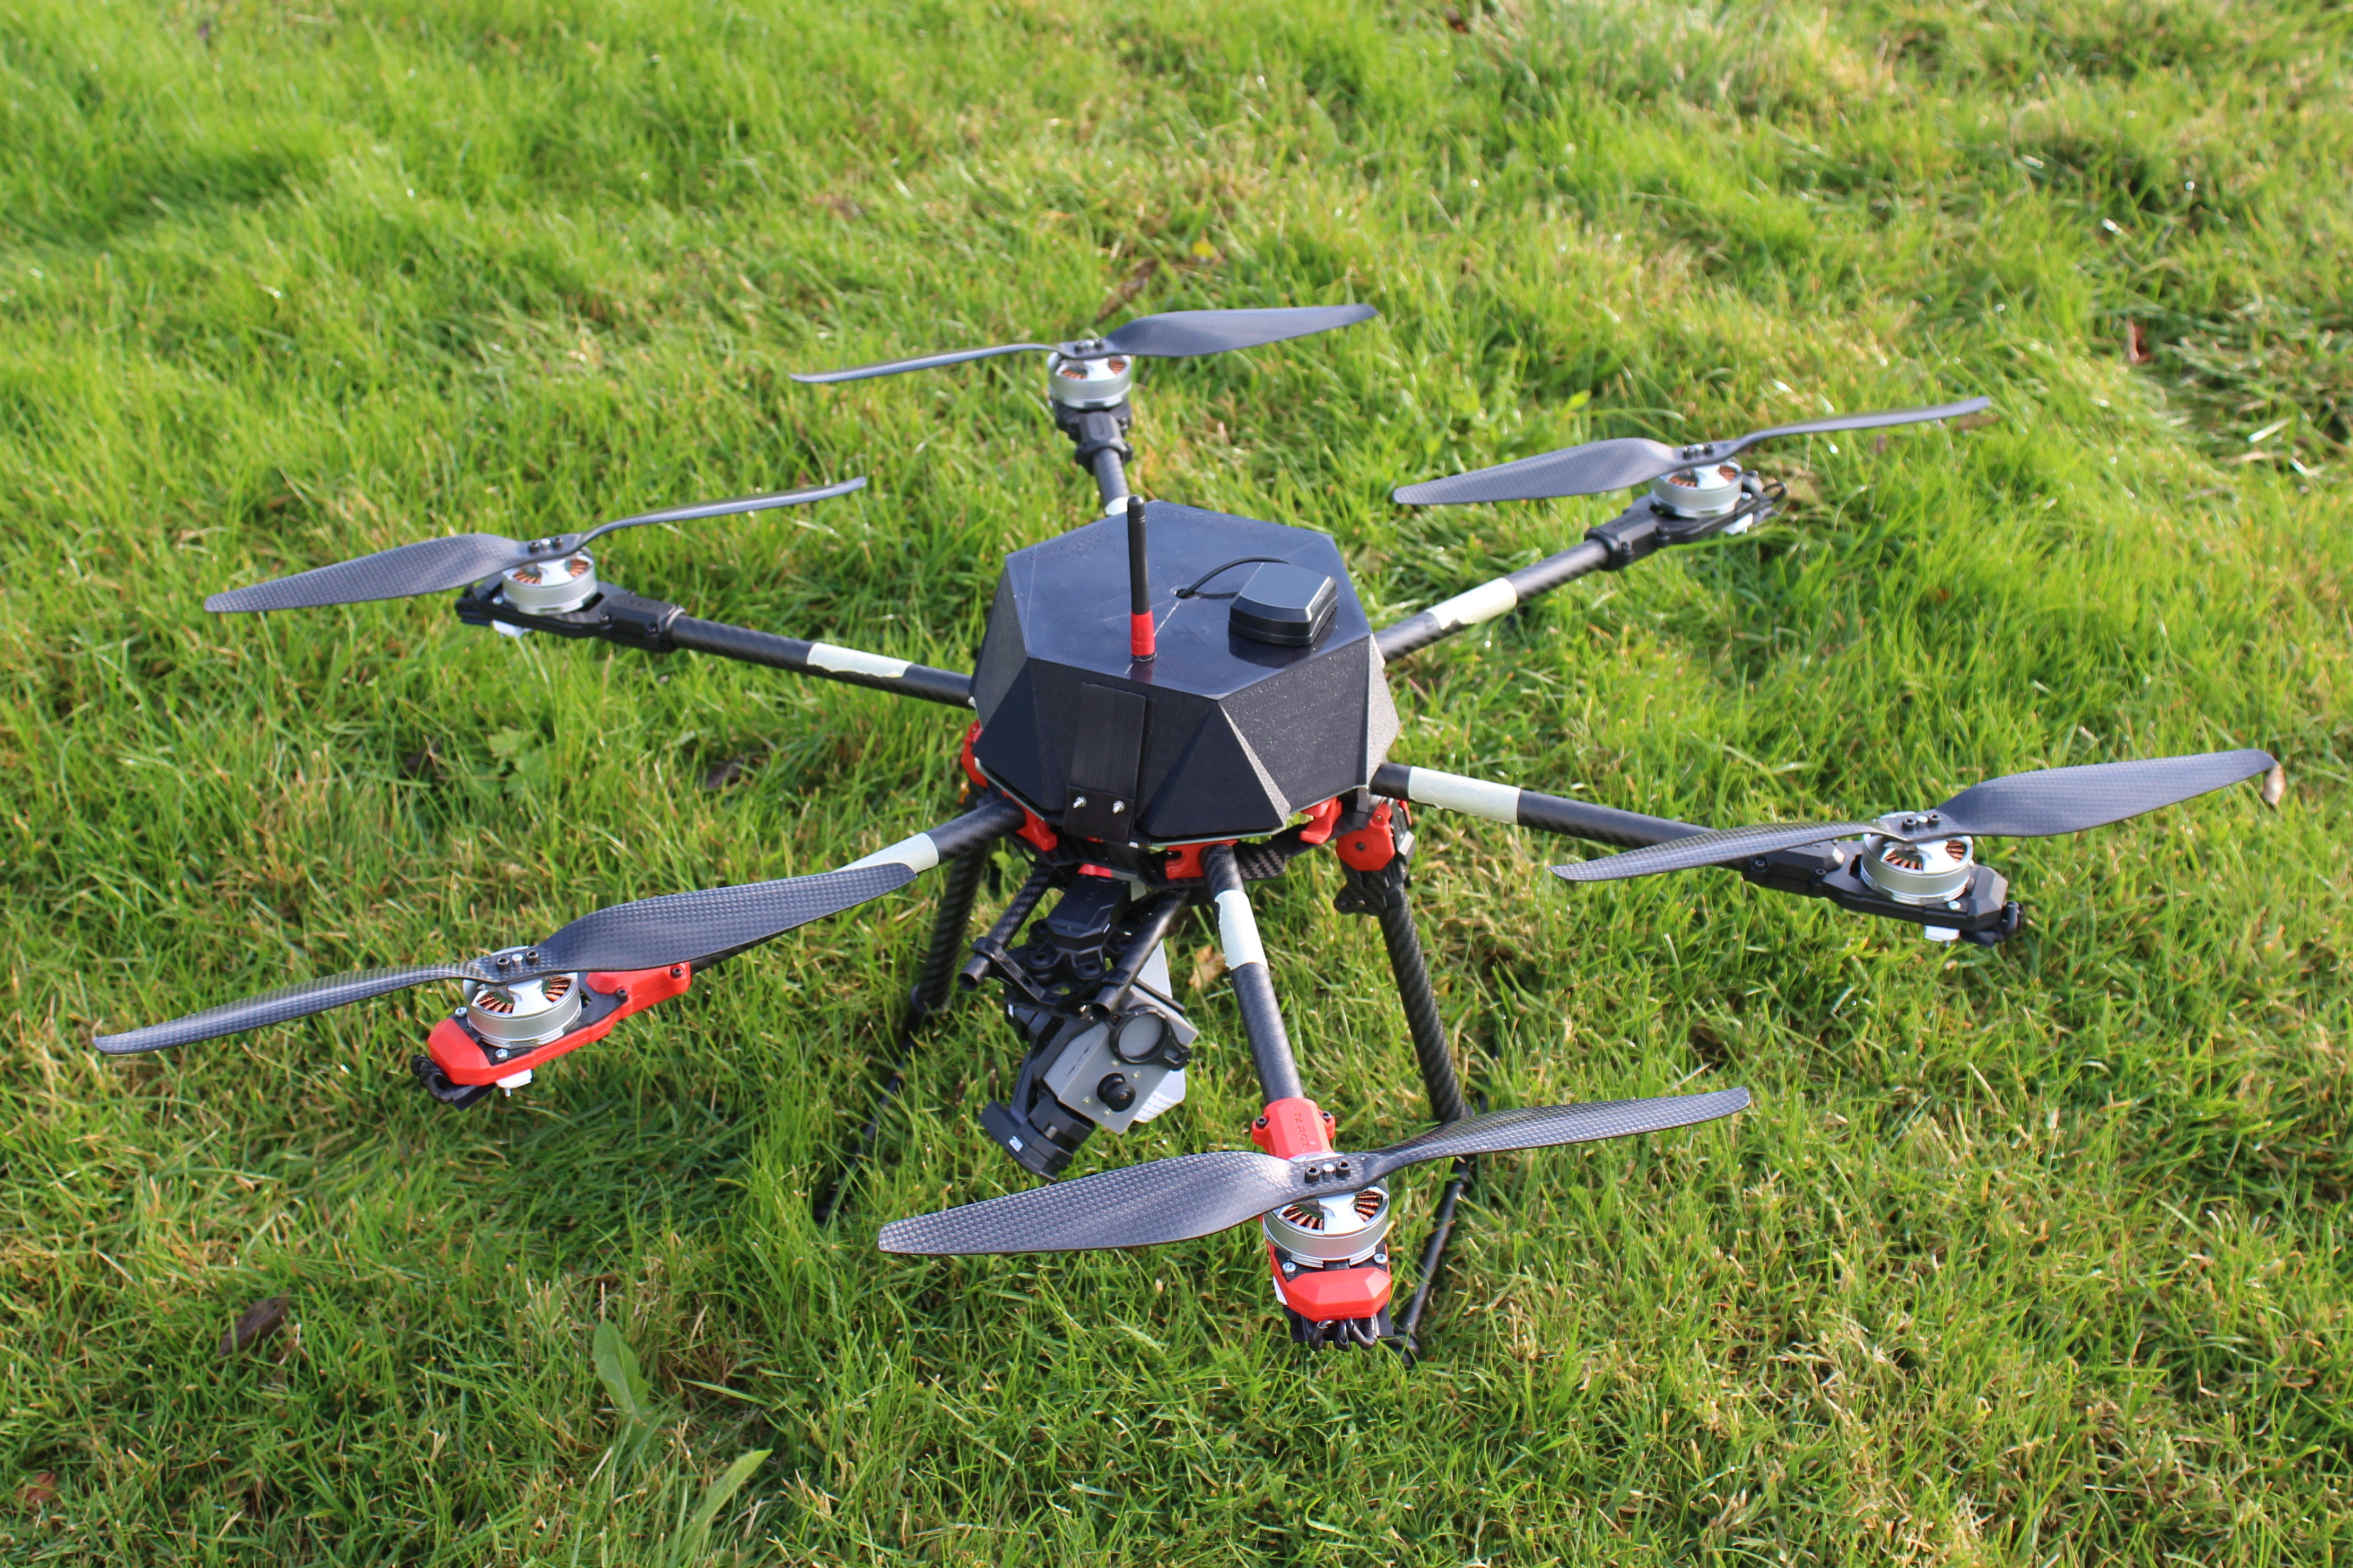
\includegraphics[width=0.45\linewidth]{jetson_drone.jpg}
        \end{tikzfigure}

        The Raspberry Pi runs a version of Raspbian Linux that is adapted for the Navio 2 hat. Together these create a flight controller, which communicates with the companion board via ROS using Ethernet over USB.
        The companion board analyzes video from the camera to detect the landing pad, aims the camera at the detected marker(s), estimates the pose of the drone relative to the landing pad, and then sends a target position to the flight controller.
        In autonomous flight mode, the flight controller flies the drone towards the target position in order to safely approach the landing pad.
        The two drones differ in their companion boards: one has an NVIDIA Jetson Nano, and the other has a Google Coral Dev.
    }

    \column{0.33}
    \block{3D-Printed Components}
    {
        \normalsize
        A canopy from Thingiverse was 3D printed to cover the electronics.
        Component mounting plates were designed in OpenSCAD and provide a flat, secure surface to mount the electronics to the drone, as well as a hinge for the canopy.
        The camera cases also provide a way to mount the camera modules in the gimbal.

        \begin{tikzfigure}[Top right to bottom left - canopy, component mounting plate, Coral camera case, Jetson Nano camera case.]
            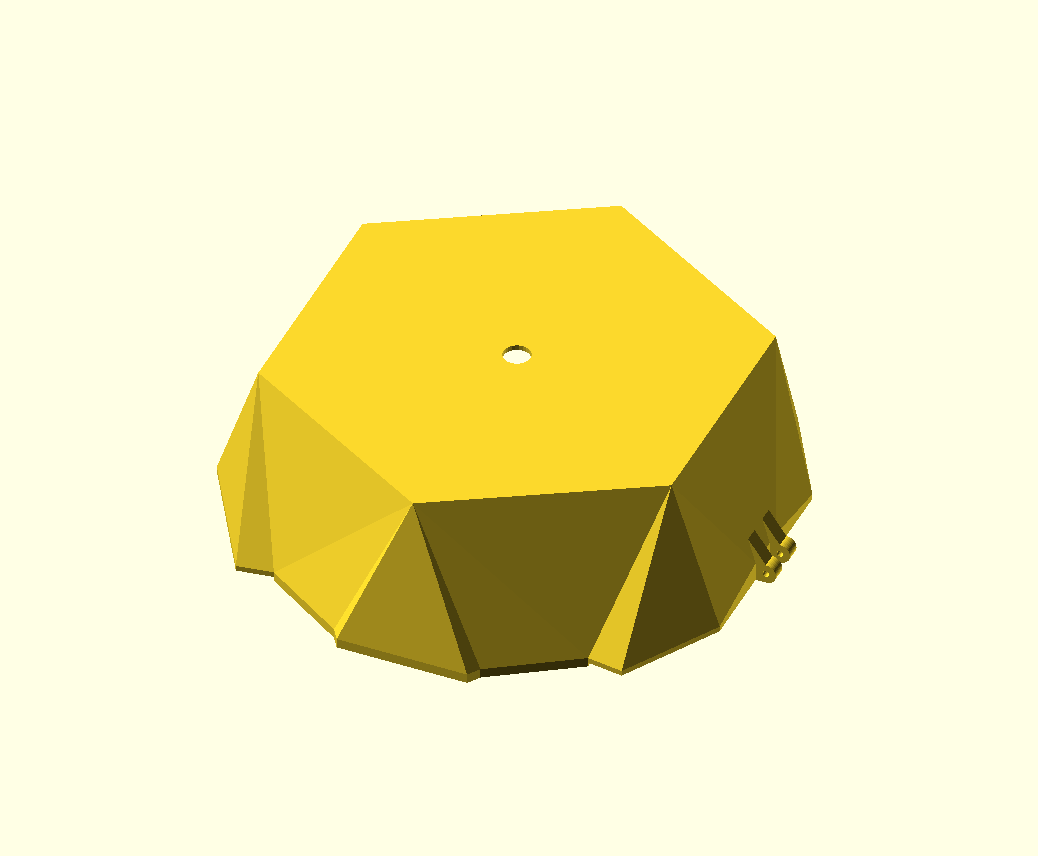
\includegraphics[width=0.4\linewidth]{canopy.png}
            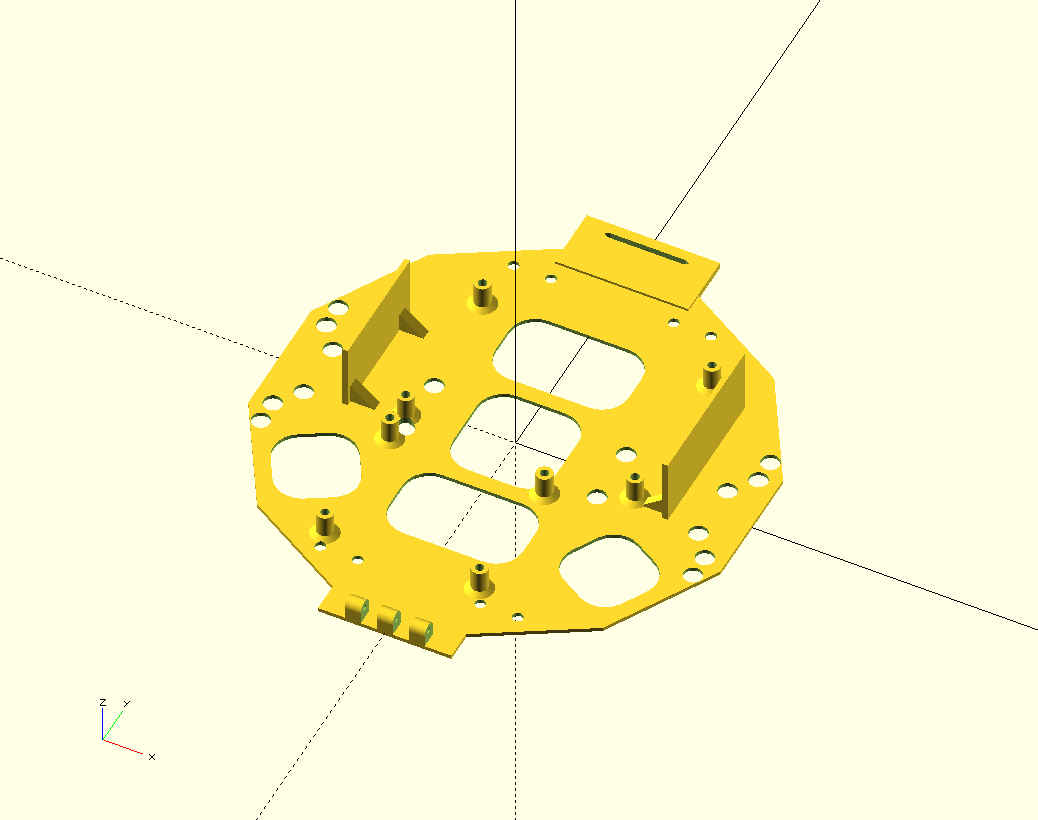
\includegraphics[width=0.4\linewidth]{component_mounting_plate}
            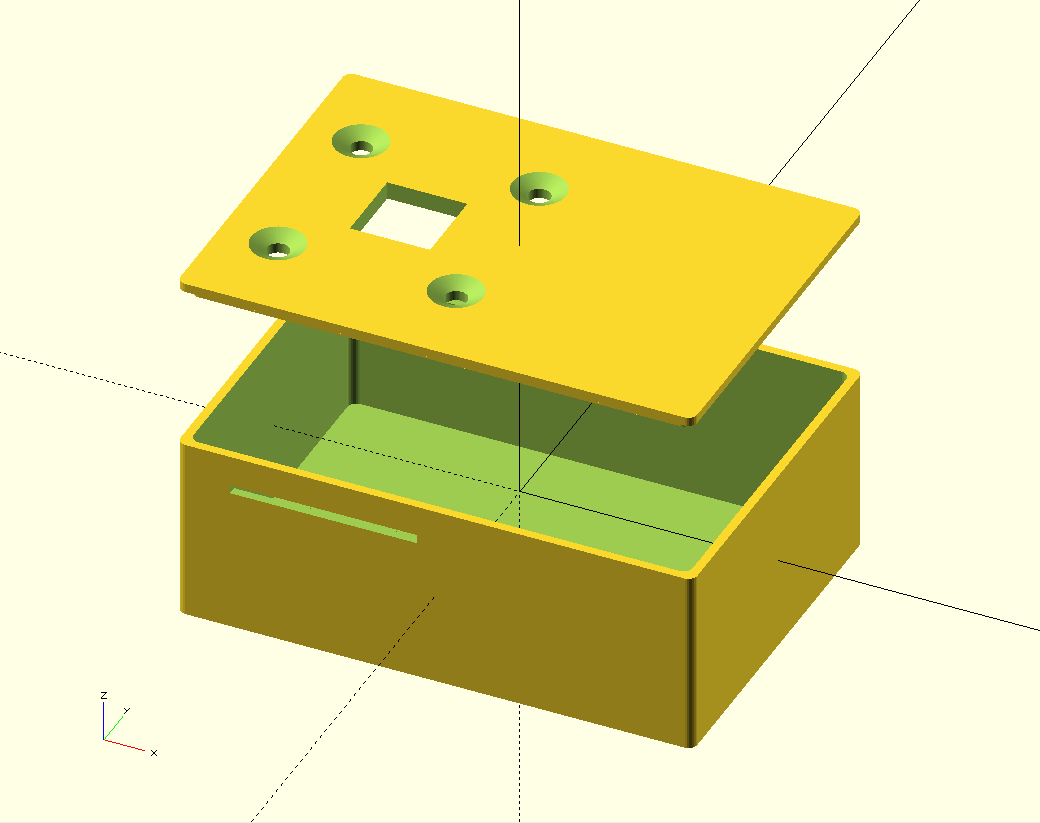
\includegraphics[width=0.4\linewidth]{coral_case.png}
            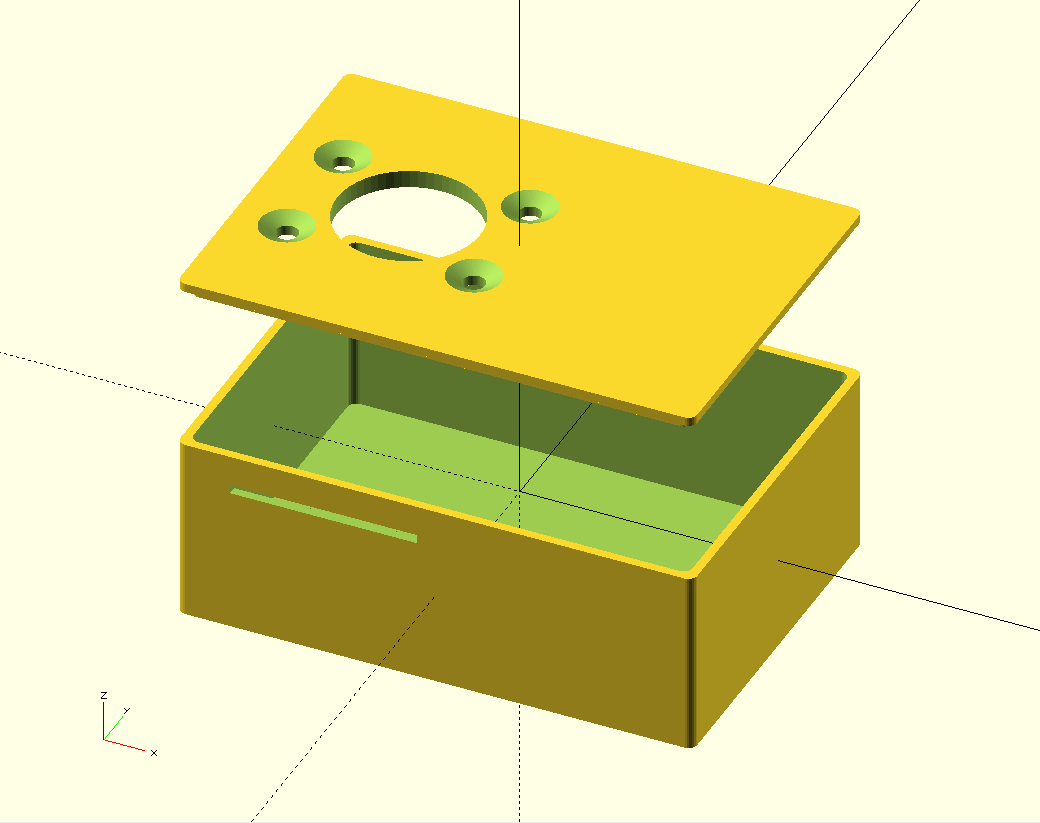
\includegraphics[width=0.4\linewidth]{nano_case.png}
        \end{tikzfigure}
    }

    \block{Landing Pad}{
        \normalsize
        \begin{minipage}[t]{0.7\linewidth}
            Fiducial markers (top: April Tag, bottom: WhyCon) allow the drone to determine its position relative to the landing pad using only a normal RGB camera.
            The larger WhyCon marker is easier for the system to recognize at long range, while the April Tag marker provides more accurate pose estimates at close range.
            The April Tag marker is positioned in front of the WhyCon marker in order to keep it in the field of view of the camera at close range.
            The drone touches down in the center of the WhyCon marker.
        \end{minipage}
        \begin{adjustbox}{valign=t}
            \begin{minipage}[t]{0.28\linewidth}
                \vspace{-1cm}
                \begin{tikzfigure}[Landing Pad]
                    \fbox{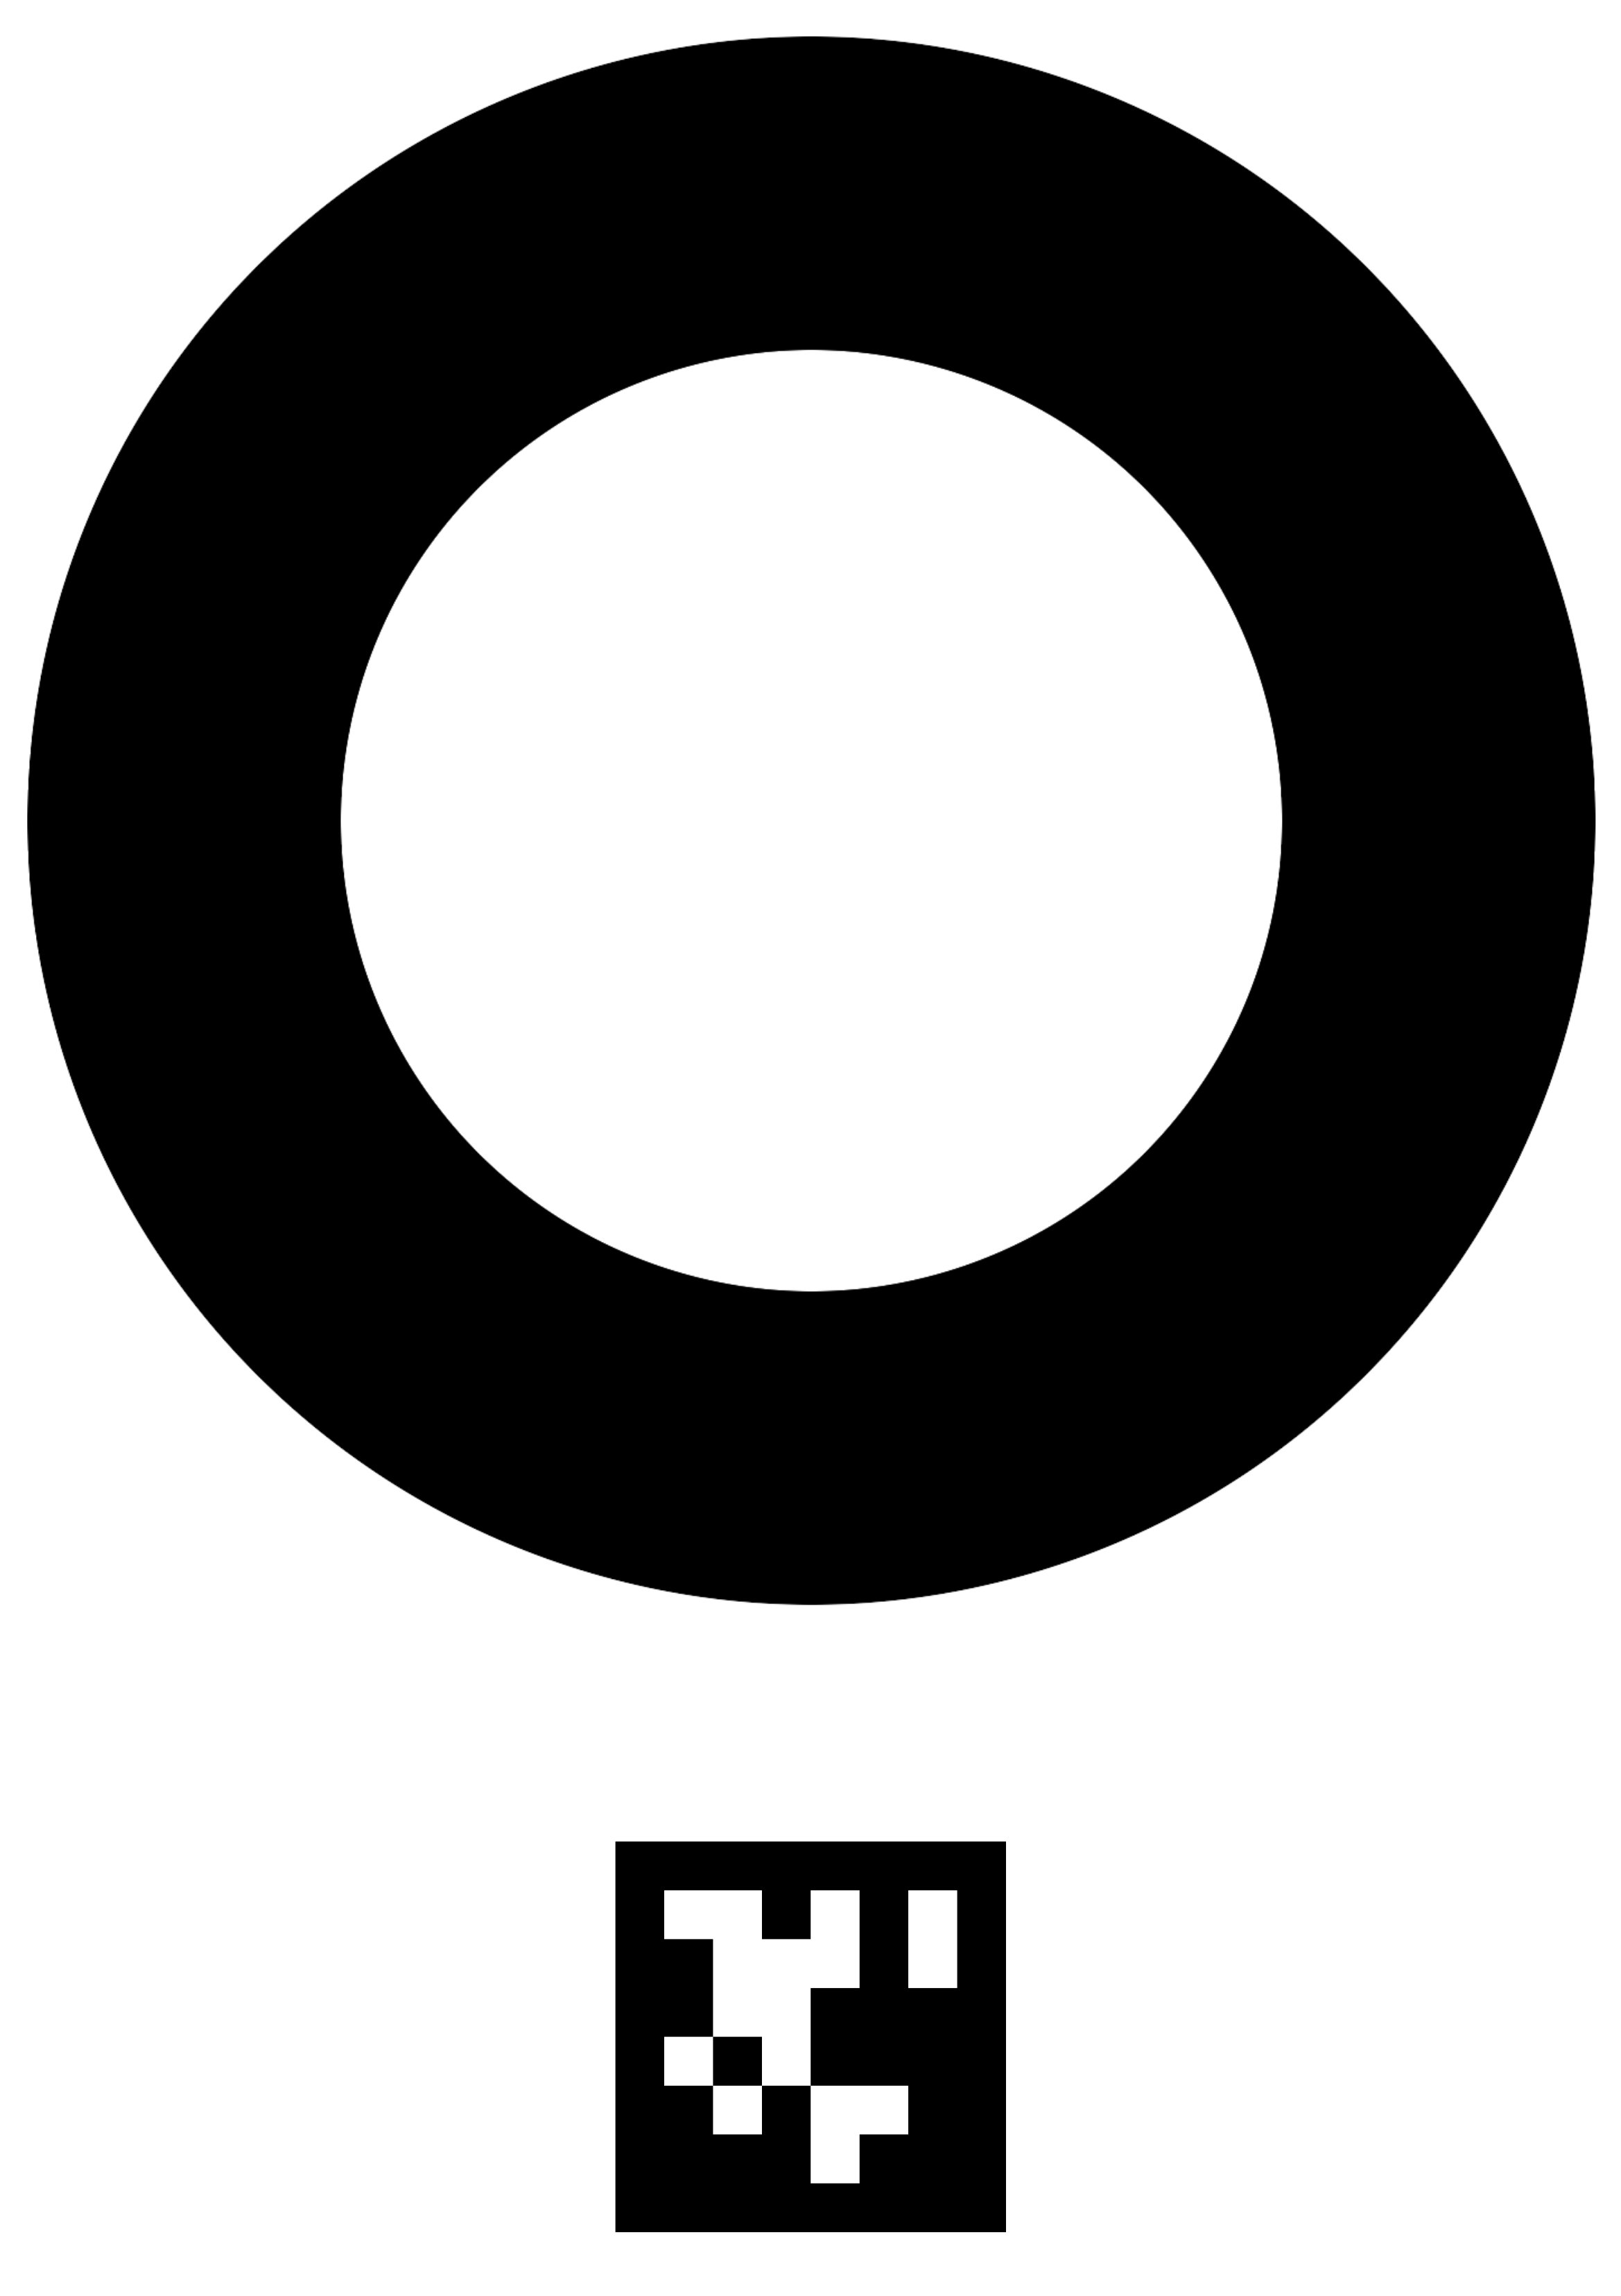
\includegraphics[angle=180, width=\linewidth]{landing_pad.png}}
                \end{tikzfigure}
            \end{minipage}
        \end{adjustbox}
    }

    \column{0.33}
    \block{Performance}
    {
        \normalsize
        Both drones have stable and reliable performance even in high wind, with safe flight times of roughly 15 minutes.
        They have enough power to lift additional sensors/electronics.
        The April Tag system was computationally heavy, especially for this embedded scenario, and was therefore replaced by the WhyCon system entirely.
        The cameras are able to aim at the landing pad reliably in a laboratory setting, however the Jetson Nano had power issues in field testing.
        The Google Coral drone was able to reliably aim the camera, generate position targets and approach the landing pad autonomously.
        Because of an issue with the WhyCon marker system, the pose estimation was inaccurate at close range and therefore landing was aborted at the last minute.
        However, this issue is not major and will be addressed in future work.

        \begin{tikzfigure}[Drone in Flight (Scan QR code in top right for video!)]
            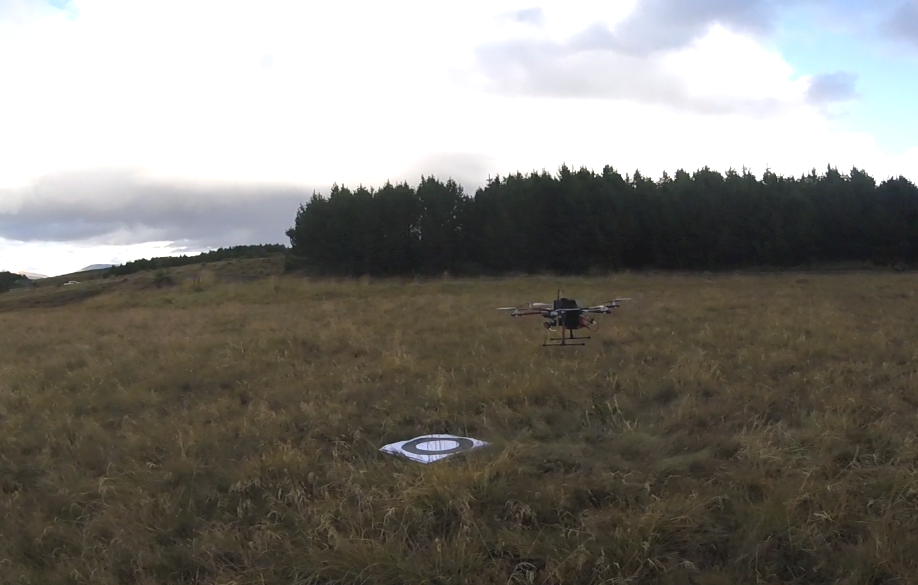
\includegraphics[width=0.9\linewidth]{drone_in_flight.png}
        \end{tikzfigure}
    }
    
    \block{Future Work}
    {
        \normalsize
        The next step is to fix the issue with pose estimation at close range.
        One possible solution is to attempt to fix the WhyCon system itself.
        Another solution is to use existing deep learning models such as EfficientPose or PoseCNN to create a new pose estimation system, as the companion boards are designed for embedded deep learning tasks.
        We will then have a good setup to re-test autonomous landing, and to continue testing more advanced drone tasks.
    }
\end{columns}
\end{document}